% Ch8 self-study -- "I do / You do" ladder for Zumdahl 8.1-8.13, four
% YOUR TURN questions per worked example. Deliberately the longest in the
% series (ten ladders) and the most illustrated (seven TikZ figures),
% because bonding is where a picture does work that prose cannot.
%
% LANGUAGE CONVENTION, with a distinction that matters here:
%  - "octet" IS legitimate in Lewis-structure work; it is the rule being
%    applied, and ladders 6-9 use it correctly.
%  - "octet / wants to be stable" is FORBIDDEN as an explanation of a
%    trend or an energy. Ladders 3-5 explain those Coulombically, and
%    ladder 4 flags the distinction explicitly.
\documentclass{apchem-worksheet}

\apcunitword{Chapter}
\apcunit{8}
\apcunittitle{Bonding: General Concepts}
\apcdoctitle{Self-Study \textbullet\ Chapter 8, I~do / You~do}
\apcsubtitle{Zumdahl \S8.1--8.13 \textbullet\ PDF pp.\ 390--445 \textbullet\ ten ladders, four questions each}

\begin{document}
\apctitleblock

\begin{apcnote}[How to use these notes --- read this first]
Each skill is a \textbf{ladder}: a fully worked example in the
solid-framed box, then \textbf{four} YOUR TURN questions in the dashed
box --- same skill, new numbers, no help.

\begin{enumerate}[leftmargin=*,itemsep=0.15em]
  \item \textbf{Work all four} before checking anything.
  \item Check against the gray \emph{check:} line. All four right on the
        first try earns the tick on the tracker (last page).
  \item Any misses: re-read the worked example, then redo the missed ones
        from a blank page.
\end{enumerate}

\textbf{This is the longest chapter in the book, and the most drawable.}
Ten ladders here, with a figure for every idea that has a shape. Draw
each figure yourself as you read it --- bonding is the one topic where
copying the picture \emph{is} the studying.

\textbf{One caution about the word ``octet''.} In Ladders 6--9 it is the
rule you are applying, and using it is correct. In Ladders 3--5 it is
\emph{not} an explanation: lattice energies, ion sizes, and bond
strengths are explained by \textbf{Coulomb's law} --- charge, distance,
shielding. Saying an ion forms ``because it wants a full shell'' names
the pattern instead of explaining it, and earns nothing.
\end{apcnote}

% =====================================================================
\section*{\sffamily Ladder 1 \textbullet\ Bond type from
electronegativity}
\zsec{8.1--8.2}

\term{Electronegativity} is an atom's pull on the electrons in a bond.
It rises across a period and falls down a group --- for the Coulombic
reasons from Chapter 7 --- so fluorine (4.0) is the highest and the
alkali metals the lowest.

The \emph{difference} between two bonded atoms decides the bond type:

\begin{center}
\begin{tikzpicture}[font=\sffamily\footnotesize]
  \draw[thick,-{Stealth[length=3mm]}] (0,0) -- (12.4,0);
  \foreach \x/\l in {0/0, 4/0.4, 8/1.7, 12/2.5+} {
    \draw[thick] (\x,0.14) -- (\x,-0.14);
    \node[below] at (\x,-0.18) {$\Delta$EN $=\l$};
  }
  \fill[apcgray!18] (0,0.18) rectangle (4,0.95);
  \fill[apcgray!38] (4,0.18) rectangle (8,0.95);
  \fill[apcgray!62] (8,0.18) rectangle (12,0.95);
  \node[align=center] at (2,0.57) {nonpolar\\covalent};
  \node[align=center] at (6,0.57) {polar\\covalent};
  \node[align=center] at (10,0.57) {ionic};
  \node[below=0.5cm] at (2,-0.2) {\ce{Cl2}, \ce{C-H}};
  \node[below=0.5cm] at (6,-0.2) {\ce{H-Cl}, \ce{O-H}};
  \node[below=0.5cm] at (10,-0.2) {\ce{NaCl}, \ce{MgO}};
\end{tikzpicture}
\end{center}

The boundaries are \emph{guidelines}, not laws --- bonding is a
continuum, and 1.7 is a convention rather than a cliff. A faster rule of
thumb: metal $+$ nonmetal is ionic, nonmetal $+$ nonmetal is covalent.

\begin{workedexample}[I do: classifying four bonds]
Electronegativities: H 2.1, C 2.5, N 3.0, O 3.5, F 4.0, Cl 3.0,
Na 0.9, Mg 1.2.

\begin{center}
\renewcommand{\arraystretch}{1.2}
\begin{tabular}{@{}llll@{}}
\hline
\textbf{Bond} & \textbf{$\Delta$EN} & \textbf{Type} &
  \textbf{Which atom is $\delta-$?} \\
\hline
\ce{H-F}  & $4.0-2.1 = 1.9$ & polar covalent (nearly ionic) & F \\
\ce{C-H}  & $2.5-2.1 = 0.4$ & essentially nonpolar & C, barely \\
\ce{Na-Cl}& $3.0-0.9 = 2.1$ & ionic & Cl (a full \ce{Cl-}) \\
\ce{O-O}  & $3.5-3.5 = 0$   & nonpolar covalent & neither \\
\hline
\end{tabular}
\end{center}

\textbf{Two things to notice.} \ce{H-F} at 1.9 sits just past the ionic
boundary yet HF is a molecular gas --- which is exactly why the number
is a guideline. And the \ce{C-H} bond, at 0.4, is treated as nonpolar
throughout organic chemistry; that approximation is why hydrocarbons do
not dissolve in water.
\end{workedexample}

\begin{yourturn}[YOUR TURN 1 --- four questions]
Use the electronegativities above, plus S 2.5, Br 2.8, Al 1.5.
\begin{enumerate}[leftmargin=*,itemsep=0.5em]
  \item Classify \ce{N-H} and say which atom carries $\delta-$.
        \workspace[1.4cm]
  \item Classify \ce{Mg-O}. \workspace[1.2cm]
  \item Rank \ce{C-F}, \ce{C-O}, \ce{C-N} by increasing bond polarity.
        \workspace[1.6cm]
  \item \ce{H-Cl} and \ce{H-F} are both polar. Which is more polar, and
        why? \workspace[1.4cm]
\end{enumerate}
\selfcheck{(a) polar covalent, $\Delta$EN $= 0.9$; N is $\delta-$ \quad
(b) ionic, $\Delta$EN $= 2.3$ \quad (c) \ce{C-N} $<$ \ce{C-O} $<$
\ce{C-F} \quad (d) \ce{H-F} --- larger $\Delta$EN}
\keyonly{\begin{apcanswer}(a) $3.0 - 2.1 = 0.9$: \textbf{polar
covalent}, with \textbf{N} the more electronegative atom and therefore
$\delta-$. (b) $3.5 - 1.2 = 2.3$: \textbf{ionic} --- a metal with a
nonmetal, as the shortcut also predicts. (c) $\Delta$EN $= 0.5$, 1.0,
1.5 respectively, so \textbf{\ce{C-N} $<$ \ce{C-O} $<$ \ce{C-F}}.
(d) \textbf{\ce{H-F}}: $\Delta$EN 1.9 against 0.9. Fluorine pulls the
shared pair much further toward itself, giving a larger partial
charge separation.\end{apcanswer}}
\end{yourturn}

% =====================================================================
\section*{\sffamily Ladder 2 \textbullet\ Dipole moments and molecular
shape}
\zsec{8.3}

A polar \emph{bond} does not guarantee a polar \emph{molecule}. Bond
dipoles are vectors: they can cancel.

\begin{center}
\begin{tikzpicture}[font=\sffamily\footnotesize,
                    dip/.style={-{Stealth[length=2.4mm]}, thick}]
  % --- HF: single polar bond ---
  \node at (0,1.35) {\textbf{\ce{HF}} --- polar};
  \node (h1) at (-0.7,0.4) {H};
  \node (f1) at (0.7,0.4) {F};
  \draw[thick] (h1) -- (f1);
  \draw[dip] (-0.55,-0.15) -- (0.55,-0.15);
  \node at (0,-0.6) {one dipole, nothing to cancel it};
  \node at (0,-1.05) {net $\mu \neq 0$};

  % --- CO2: linear, cancels ---
  \begin{scope}[xshift=4.9cm]
    \node at (0,1.35) {\textbf{\ce{CO2}} --- nonpolar};
    \node (o1) at (-1.05,0.4) {O};
    \node (c1) at (0,0.4) {C};
    \node (o2) at (1.05,0.4) {O};
    \draw[thick] (o1) -- (c1); \draw[thick] (c1) -- (o2);
    \draw[dip] (-0.15,-0.15) -- (-0.95,-0.15);
    \draw[dip] (0.15,-0.15) -- (0.95,-0.15);
    \node at (0,-0.6) {equal and opposite};
    \node at (0,-1.05) {net $\mu = 0$};
  \end{scope}

  % --- H2O: bent, adds ---
  \begin{scope}[xshift=9.8cm]
    \node at (0,1.35) {\textbf{\ce{H2O}} --- polar};
    \node (ow) at (0,0.72) {O};
    \node (h2) at (-0.8,-0.05) {H};
    \node (h3) at (0.8,-0.05) {H};
    \draw[thick] (ow) -- (h2); \draw[thick] (ow) -- (h3);
    \draw[dip] (-0.62,0.05) -- (-0.12,0.55);
    \draw[dip] (0.62,0.05) -- (0.12,0.55);
    \draw[dip, apcaccent] (0,-0.45) -- (0,0.35);
    \node at (0,-0.85) {they add, upward};
    \node at (0,-1.25) {net $\mu \neq 0$};
  \end{scope}
\end{tikzpicture}
\end{center}

\textbf{The test, in two steps:} are the bonds polar? and does the
\emph{shape} let the dipoles cancel? Both must be answered.

\begin{workedexample}[I do: same bonds, opposite answers]
\ce{CO2} and \ce{H2O} both contain strongly polar bonds
($\Delta$EN $= 1.0$ and $1.4$). Why is only one of them a polar
molecule?

\textbf{\ce{CO2}} is \textbf{linear}. The two \ce{C=O} dipoles point
directly away from each other along one axis, equal in size and opposite
in direction, so their vector sum is exactly zero. The molecule is
\textbf{nonpolar} despite having two of the most polar bonds in the
chapter.

\textbf{\ce{H2O}} is \textbf{bent} at \SI{104.5}{\degree}. The two
\ce{O-H} dipoles point from each H toward the O, and because they are not
opposed they add to a net dipole pointing up through the oxygen. The
molecule is \textbf{polar} --- which is why water dissolves salts,
has a high boiling point, and lines up in a microwave.

\textbf{The generalization worth carrying:} a molecule with identical
outer atoms and \emph{no lone pairs} on the central atom is symmetric,
so its dipoles cancel. Add a lone pair --- or make the outer atoms
different --- and the symmetry breaks.
\end{workedexample}

\begin{yourturn}[YOUR TURN 2 --- four questions]
\begin{enumerate}[leftmargin=*,itemsep=0.5em]
  \item Is \ce{CCl4} (tetrahedral) polar? Explain. \workspace[1.4cm]
  \item Is \ce{NH3} (trigonal pyramidal) polar? Explain.
        \workspace[1.4cm]
  \item \ce{CH3Cl} is tetrahedral like \ce{CCl4}. Is it polar?
        \workspace[1.4cm]
  \item Can a molecule with nonpolar bonds ever be polar?
        \workspace[1.4cm]
\end{enumerate}
\selfcheck{(a) no --- symmetric, dipoles cancel \quad (b) yes --- the
lone pair breaks the symmetry \quad (c) yes --- the outer atoms differ
\quad (d) no}
\keyonly{\begin{apcanswer}(a) \textbf{No.} The four \ce{C-Cl} bonds are
polar, but they point to the corners of a tetrahedron with identical
outer atoms, so the four dipoles sum to zero. (b) \textbf{Yes.} Ammonia
has three \ce{N-H} dipoles \emph{and} a lone pair on nitrogen. The shape
is pyramidal rather than planar, so the dipoles do not cancel and the
net points through the lone pair. (c) \textbf{Yes.} The geometry is
still tetrahedral, but three outer atoms are H and one is Cl. The
\ce{C-Cl} dipole is much larger than the three \ce{C-H} dipoles opposing
it, so a net dipole survives --- symmetry of \emph{shape} is not enough;
the outer atoms must match too. (d) \textbf{No.} With no polar bonds
there are no bond dipoles to add, so the vector sum is zero no matter
what the shape is.\end{apcanswer}}
\end{yourturn}

% =====================================================================
\section*{\sffamily Ladder 3 \textbullet\ Ion sizes and isoelectronic
series}
\zsec{8.4}

Forming an ion changes the electron count but never the nuclear charge.
Everything follows from that.

\begin{itemize}[leftmargin=*,itemsep=0.15em]
  \item \textbf{Cations are smaller} than their parent atoms: electrons
        are removed, often emptying the outer shell entirely, and the
        unchanged nuclear charge now pulls on fewer electrons.
  \item \textbf{Anions are larger}: added electrons increase
        electron--electron repulsion in the valence shell while the
        nuclear charge stays put, so the cloud expands.
  \item In an \term{isoelectronic} series --- same electron count ---
        size falls as nuclear charge rises.
\end{itemize}

\begin{center}
\begin{tikzpicture}[font=\sffamily\footnotesize]
  \foreach \x/\r/\l/\z in {0/0.85/\ce{N^3-}/7, 2.3/0.72/\ce{O^2-}/8,
                           4.6/0.60/\ce{F-}/9, 6.9/0.44/\ce{Na+}/11,
                           9.2/0.36/\ce{Mg^2+}/12} {
    \fill[apcgray!30] (\x,0) circle (\r);
    \draw[apcgray] (\x,0) circle (\r);
    \node[circle,fill=black,inner sep=1pt] at (\x,0) {};
    \node at (\x,-1.15) {\l};
    \node at (\x,-1.55) {$Z = \z$};
  }
  \draw[-{Stealth[length=3mm]},thick] (-0.9,1.25) -- (10.1,1.25);
  \node[above,font=\sffamily\small] at (4.6,1.3)
    {all 10 electrons \textbullet\ nuclear charge rises \textbullet\
     radius falls};
\end{tikzpicture}
\end{center}

\begin{workedexample}[I do: ordering an isoelectronic series]
Rank \ce{S^2-}, \ce{Cl-}, \ce{K+}, and \ce{Ca^2+} by size, largest
first, and justify.

\textbf{First establish they are isoelectronic.} $16+2 = 18$,
$17+1 = 18$, $19-1 = 18$, $20-2 = 18$. All have 18 electrons --- the
argon configuration --- so \textbf{shielding is identical} across the
set. That is what makes the comparison clean.

\textbf{Now the only variable left is nuclear charge:} 16, 17, 19, 20.

\[ \ce{S^2-} > \ce{Cl-} > \ce{K+} > \ce{Ca^2+} \]

\textbf{Why:} each ion holds the same 18 electrons, but calcium's
\textbf{20 protons} pull them in far harder than sulfur's \textbf{16}.
More nuclear charge on an unchanged electron cloud means a smaller
radius.

\textbf{Note what the explanation did not say:} nothing about full
shells or stability. Every ion here has the same full shell --- that is
precisely the point, and it is why only Coulomb's law can distinguish
them.
\end{workedexample}

\begin{yourturn}[YOUR TURN 3 --- four questions]
\begin{enumerate}[leftmargin=*,itemsep=0.5em]
  \item Which is larger, \ce{Fe^2+} or \ce{Fe^3+}? Why?
        \workspace[1.4cm]
  \item Which is larger, \ce{Br} or \ce{Br-}? Why? \workspace[1.4cm]
  \item Rank \ce{N^3-}, \ce{O^2-}, \ce{F-} by size and justify in one
        sentence. \workspace[1.6cm]
  \item \ce{K+} and \ce{Cl-} are isoelectronic. Explain why the cation
        is the smaller one. \workspace[1.6cm]
\end{enumerate}
\selfcheck{(a) \ce{Fe^2+} \quad (b) \ce{Br-} \quad (c) \ce{N^3-} $>$
\ce{O^2-} $>$ \ce{F-} \quad (d) potassium has more protons on the same
18 electrons}
\keyonly{\begin{apcanswer}(a) \textbf{\ce{Fe^2+}}. Both have 26 protons,
but \ce{Fe^3+} has one fewer electron, so the same nuclear charge is
shared among fewer electrons and pulls each more tightly. (b)
\textbf{\ce{Br-}}. The added electron does not change the 35 protons but
does increase repulsion within the valence shell, expanding the cloud.
(c) \textbf{\ce{N^3-} $>$ \ce{O^2-} $>$ \ce{F-}} --- all have 10
electrons and identical shielding, so the rising nuclear charge (7, 8, 9)
contracts them in that order. (d) Both hold 18 electrons with the same
shielding, but potassium has \textbf{19 protons} against chlorine's
\textbf{17}. The greater nuclear charge draws the identical electron
cloud in more tightly, so \ce{K+} is smaller.\end{apcanswer}}
\end{yourturn}

% =====================================================================
\section*{\sffamily Ladder 4 \textbullet\ Lattice energy}
\zsec{8.5}

\term{Lattice energy} is the energy released when gaseous ions come
together into a crystal --- large and negative, and the reason ionic
solids have high melting points. It is pure Coulomb's law:

\[ E \;\propto\; \frac{Q_1 Q_2}{r} \]

\textbf{Charge dominates.} Doubling a charge doubles the numerator;
changing ionic radius moves the denominator only modestly. So when
comparing two compounds, look at charges first and only use size as a
tie-breaker.

\begin{workedexample}[I do: two comparisons, charge then size]
\textbf{(a) Which has the larger lattice energy, \ce{NaCl} or
\ce{MgO}?}

\ce{NaCl} pairs $1+$ with $1-$: the product $Q_1Q_2$ has magnitude 1.
\ce{MgO} pairs $2+$ with $2-$: magnitude 4. On top of that, \ce{Mg^2+}
and \ce{O^2-} are both smaller than \ce{Na+} and \ce{Cl-}, shrinking $r$
as well.

\textbf{\ce{MgO}}, by a wide margin --- roughly four times, and its
melting point (\SI{2852}{\celsius}) towers over sodium chloride's
(\SI{801}{\celsius}). Both factors push the same way.

\textbf{(b) Which has the larger lattice energy, \ce{NaCl} or
\ce{NaBr}?}

Here the charges are identical ($1+$, $1-$), so charge cannot decide it
and size becomes the tie-breaker. Bromide is larger than chloride, so
$r$ is larger and the energy smaller: \textbf{\ce{NaCl}}.

\textbf{The order of operations:} compare $Q_1Q_2$ first. Only if it
ties do you compare $r$. Reversing that order is how students conclude
that \ce{LiF} beats \ce{MgO}.
\end{workedexample}

\begin{yourturn}[YOUR TURN 4 --- four questions]
\begin{enumerate}[leftmargin=*,itemsep=0.5em]
  \item Larger lattice energy: \ce{KCl} or \ce{CaO}? Why?
        \workspace[1.4cm]
  \item Larger lattice energy: \ce{LiF} or \ce{KF}? Why?
        \workspace[1.4cm]
  \item Larger lattice energy: \ce{MgO} or \ce{MgS}? Why?
        \workspace[1.4cm]
  \item Which melts higher, \ce{NaF} or \ce{MgF2}? Connect your answer
        to lattice energy. \workspace[1.6cm]
\end{enumerate}
\selfcheck{(a) \ce{CaO} \quad (b) \ce{LiF} \quad (c) \ce{MgO} \quad
(d) \ce{MgF2} --- larger cation charge, larger lattice energy}
\keyonly{\begin{apcanswer}(a) \textbf{\ce{CaO}}: charges $2+/2-$ give
$Q_1Q_2 = 4$ against \ce{KCl}'s 1, and the ions are smaller as well.
(b) \textbf{\ce{LiF}}: the charges tie at $1+/1-$, so size decides, and
\ce{Li+} is much smaller than \ce{K+}, giving a smaller $r$. (c)
\textbf{\ce{MgO}}: charges tie at $2+/2-$, so size decides, and oxide is
smaller than sulfide. (d) \textbf{\ce{MgF2}}. Its \ce{Mg^2+} carries
twice the charge of \ce{Na+}, so $Q_1Q_2$ is 2 rather than 1 and the
lattice energy is substantially larger. More energy is needed to pull the
lattice apart, which is exactly what a higher melting point
measures.\end{apcanswer}}
\end{yourturn}

% =====================================================================
\section*{\sffamily Ladder 5 \textbullet\ Bond energies and $\Delta H$}
\zsec{8.8}

\textbf{Breaking a bond always costs energy; forming one always releases
it.} There are no exceptions, and the whole calculation follows:

\[ \boxed{\;\Delta H \approx \sum(\text{bonds broken})
   - \sum(\text{bonds formed})\;} \]

\begin{center}
\begin{tikzpicture}[font=\sffamily\footnotesize]
  \draw[-{Stealth[length=3mm]}] (0,0) -- (0,4.3) node[above] {enthalpy};
  % reactants
  \draw[very thick] (0.6,1.3) -- (2.4,1.3);
  \node[align=center] at (1.5,0.85) {reactants\\\ce{H2 + Cl2}};
  % atoms at top
  \draw[very thick] (4.2,3.6) -- (6.6,3.6);
  \node[align=center] at (5.4,4.0) {free atoms};
  % products
  \draw[very thick] (8.4,0.35) -- (10.2,0.35);
  \node[align=center] at (9.3,-0.15) {products\\\ce{2HCl}};
  % arrows
  \draw[-{Stealth[length=2.6mm]},thick] (2.4,1.3) -- (4.2,3.6);
  \node[above left,align=center] at (3.6,2.6) {break\\$+671$};
  \draw[-{Stealth[length=2.6mm]},thick] (6.6,3.6) -- (8.4,0.35);
  \node[above right,align=center] at (7.3,2.3) {form\\$-854$};
  \draw[dashed,apcgray] (2.4,1.3) -- (10.4,1.3);
  \draw[-{Stealth[length=2.6mm]},thick,apcaccent] (10.6,1.3) -- (10.6,0.35);
  \node[right,align=left] at (10.75,0.8) {net\\$\Delta H = -183$};
\end{tikzpicture}
\end{center}

Uphill to tear everything apart, further downhill to build the products.
The net is the difference --- and the answer is an \emph{estimate},
because a tabulated bond energy is an average over many molecules.

\begin{workedexample}[I do: hydrogen chloride, then a reality check]
Estimate $\Delta H$ for $\ce{H2(g) + Cl2(g) -> 2HCl(g)}$.
Bond energies (kJ/mol): \ce{H-H} 432, \ce{Cl-Cl} 239, \ce{H-Cl} 427.

\textbf{Bonds broken} --- one of each reactant bond:
\[ 432 + 239 = \SI{671}{\kilo\joule} \]

\textbf{Bonds formed} --- two \ce{H-Cl}:
\[ 2(427) = \SI{854}{\kilo\joule} \]

\textbf{Net:}
\[ \Delta H \approx 671 - 854 = \mathbf{-183~kJ} \]

\textbf{Reality check.} The measured value is \SI{-184.6}{\kilo\joule}
--- agreement to under 1\%, which is unusually good. Expect 5--10\% for
larger molecules, because the tables average a bond over every compound
it appears in, and a \ce{C-H} bond in methane is not identical to one in
ethanol.

\textbf{Sign sanity:} more energy came out than went in, so the reaction
is exothermic and $\Delta H$ is negative. If your answer is positive for
a combustion, you have reversed the subtraction.
\end{workedexample}

\begin{yourturn}[YOUR TURN 5 --- four questions]
Bond energies (kJ/mol): \ce{C-H} 413, \ce{O=O} 495, \ce{C=O} 799,
\ce{O-H} 467, \ce{N#N} 941, \ce{H-H} 432, \ce{N-H} 391.
\begin{enumerate}[leftmargin=*,itemsep=0.5em]
  \item Estimate $\Delta H$ for
        $\ce{CH4(g) + 2O2(g) -> CO2(g) + 2H2O(g)}$. \workspace[2.4cm]
  \item Estimate $\Delta H$ for
        $\ce{N2(g) + 3H2(g) -> 2NH3(g)}$. \workspace[2.2cm]
  \item The measured value for (a) is \SI{-802}{\kilo\joule}. Why does
        the estimate differ? \workspace[1.6cm]
  \item Is breaking the \ce{N#N} bond endothermic or exothermic, and what
        does its size (941) tell you about nitrogen gas?
        \workspace[1.6cm]
\end{enumerate}
\selfcheck{(a) \SI{-824}{\kilo\joule} \quad (b) \SI{-109}{\kilo\joule}
\quad (c) tabulated bond energies are averages \quad (d) endothermic;
\ce{N2} is very unreactive}
\keyonly{\begin{apcanswer}(a) Broken: $4(413) + 2(495) = 1652 + 990 =
2642$. Formed: $2(799) + 4(467) = 1598 + 1868 = 3466$.
$\Delta H \approx 2642 - 3466 = \mathbf{-824}$~kJ.
(b) Broken: $941 + 3(432) = 941 + 1296 = 2237$. Formed:
$6(391) = 2346$. $\Delta H \approx \mathbf{-109}$~kJ.
(c) Because a tabulated bond energy is an \textbf{average} of that bond
across many different molecules, not its exact value in this one. The
22 kJ gap --- under 3\% --- is typical. (d) \textbf{Endothermic}:
breaking any bond costs energy. At 941 kJ/mol it is one of the strongest
bonds known, which is why \ce{N2} is almost inert and why industrial
ammonia synthesis needs high temperature, high pressure and a
catalyst.\end{apcanswer}}
\end{yourturn}

% =====================================================================
\section*{\sffamily Ladder 6 \textbullet\ Drawing Lewis structures}
\zsec{8.9--8.10}

Five steps, in this order, every time:

\begin{enumerate}[leftmargin=*,itemsep=0.15em]
  \item Count \textbf{total valence electrons} (add for a negative
        charge, subtract for a positive one).
  \item Place the \textbf{least electronegative atom} at the centre ---
        never hydrogen, which forms only one bond.
  \item Join everything with \textbf{single bonds}, then subtract
        $2$ electrons per bond.
  \item Distribute the remainder as \textbf{lone pairs on the outer
        atoms} first, completing their octets.
  \item If the centre is short of an octet, \textbf{make multiple bonds}
        by moving outer lone pairs into the bond.
\end{enumerate}

\begin{center}
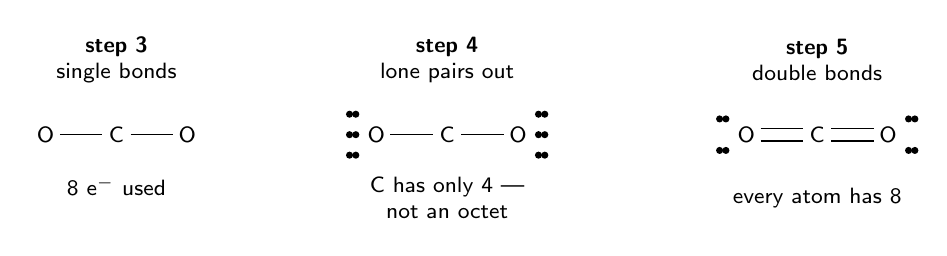
\begin{tikzpicture}[font=\sffamily\footnotesize, node distance=0.4cm]
  \node[align=center] at (0,1.45) {\textbf{step 3}\\single bonds};
  \node at (-0.9,0.5) {O}; \node at (0,0.5) {C}; \node at (0.9,0.5) {O};
  \draw (-0.72,0.5) -- (-0.18,0.5); \draw (0.18,0.5) -- (0.72,0.5);
  \node at (0,-0.15) {8 e$^-$ used};

  \begin{scope}[xshift=4.2cm]
    \node[align=center] at (0,1.45) {\textbf{step 4}\\lone pairs out};
    \node at (-0.9,0.5) {O}; \node at (0,0.5) {C}; \node at (0.9,0.5) {O};
    \draw (-0.72,0.5) -- (-0.18,0.5); \draw (0.18,0.5) -- (0.72,0.5);
    \foreach \d in {-1,1} {
      \foreach \y in {0.24,0.5,0.76} {
        \fill (\d*0.9 + \d*0.26, \y) circle (0.045);
        \fill (\d*0.9 + \d*0.34, \y) circle (0.045);}}
    \node[align=center] at (0,-0.3) {C has only 4 --- \\not an octet};
  \end{scope}

  \begin{scope}[xshift=8.9cm]
    \node[align=center] at (0,1.45) {\textbf{step 5}\\double bonds};
    \node at (-0.9,0.5) {O}; \node at (0,0.5) {C}; \node at (0.9,0.5) {O};
    \draw (-0.72,0.58) -- (-0.18,0.58); \draw (-0.72,0.42) -- (-0.18,0.42);
    \draw (0.18,0.58) -- (0.72,0.58);   \draw (0.18,0.42) -- (0.72,0.42);
    \foreach \d in {-1,1} {
      \foreach \y in {0.30,0.70} {
        \fill (\d*0.9 + \d*0.26, \y) circle (0.045);
        \fill (\d*0.9 + \d*0.34, \y) circle (0.045);}}
    \node at (0,-0.3) {every atom has 8};
  \end{scope}
\end{tikzpicture}
\end{center}

\begin{workedexample}[I do: the nitrate ion, \ce{NO3-}]
\textbf{Step 1 --- count.} N contributes 5, each O contributes 6, and the
$1-$ charge adds one more:
\[ 5 + 3(6) + 1 = \SI{24}{electrons} \]

\textbf{Step 2 --- centre.} Nitrogen is less electronegative than oxygen,
so N sits in the middle with three O around it.

\textbf{Step 3 --- single bonds.} Three \ce{N-O} bonds use
$3 \times 2 = 6$ electrons, leaving $24 - 6 = 18$.

\textbf{Step 4 --- lone pairs outward.} Each oxygen needs three lone
pairs to reach an octet: $3 \times 6 = 18$ electrons. All 24 are now
placed.

\textbf{Step 5 --- check the centre.} Nitrogen has only the three
bonding pairs, or 6 electrons. Short of an octet, so move one lone pair
from an oxygen into a bond, making one \ce{N=O} double bond. Nitrogen now
has 8.

\textbf{Final:} one \ce{N=O} and two \ce{N-O}, with the whole thing in
brackets carrying a $1-$ charge. That the double bond could equally have
gone to any of the three oxygens is the subject of Ladder 9.

\textbf{The count is the check.} If your finished structure does not use
exactly 24 electrons, it is wrong regardless of how it looks.
\end{workedexample}

\begin{yourturn}[YOUR TURN 6 --- four questions]
\begin{enumerate}[leftmargin=*,itemsep=0.5em]
  \item Total valence electrons in \ce{CH4}, and draw it.
        \workspace[1.8cm]
  \item Total valence electrons in \ce{NH4+}, and draw it.
        \workspace[1.8cm]
  \item Draw \ce{CO} and state the bond order. \workspace[1.8cm]
  \item Draw \ce{SO2} and say how many lone pairs sit on the sulfur.
        \workspace[1.8cm]
\end{enumerate}
\selfcheck{(a) 8 \quad (b) 8 --- subtract one for the $+$ charge \quad
(c) 10 electrons, a triple bond \quad (d) 18 electrons, one lone pair on
S}
\keyonly{\begin{apcanswer}(a) $4 + 4(1) = \mathbf{8}$: four \ce{C-H}
single bonds, no lone pairs anywhere. (b) $5 + 4(1) - 1 = \mathbf{8}$ ---
\textbf{subtract} one for the positive charge. Four \ce{N-H} bonds, the
whole ion in brackets with a $+$. (c) $4 + 6 = \mathbf{10}$. A triple
bond, \ce{C#O}, with one lone pair on each atom --- \textbf{bond order
3}. (d) $6 + 2(6) = \mathbf{18}$. One \ce{S=O} and one \ce{S-O} (or
resonance between them), with \textbf{one lone pair} on sulfur, which is
what makes the molecule bent rather than
linear.\end{apcanswer}}
\end{yourturn}

% =====================================================================
\section*{\sffamily Ladder 7 \textbullet\ Exceptions to the octet rule}
\zsec{8.11}

Three kinds, and each is recognizable on sight.

\begin{center}
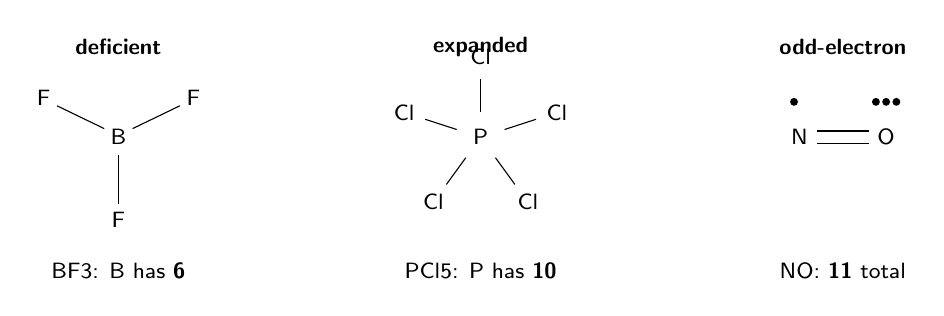
\begin{tikzpicture}[font=\sffamily\footnotesize]
  % BF3 -- electron deficient
  \node[align=center] at (0,1.7) {\textbf{deficient}};
  \node at (0,0.55) {B};
  \node at (0,-0.5) {F}; \node at (-0.95,1.05) {F}; \node at (0.95,1.05) {F};
  \draw (0,0.33) -- (0,-0.3); \draw (-0.18,0.66) -- (-0.78,0.95);
  \draw (0.18,0.66) -- (0.78,0.95);
  \node[align=center] at (0,-1.15) {\ce{BF3}: B has \textbf{6}};

  % PCl5 -- expanded
  \begin{scope}[xshift=4.6cm]
    \node[align=center] at (0,1.7) {\textbf{expanded}};
    \node at (0,0.55) {P};
    \foreach \a in {90,162,234,306,18} {
      \draw (\a:0.32) ++(0,0.55) -- ++(\a:0.42);
      \node at ([shift={(0,0.55)}]\a:1.02) {Cl};}
    \node[align=center] at (0,-1.15) {\ce{PCl5}: P has \textbf{10}};
  \end{scope}

  % NO -- odd electron
  \begin{scope}[xshift=9.2cm]
    \node[align=center] at (0,1.7) {\textbf{odd-electron}};
    \node at (-0.55,0.55) {N}; \node at (0.55,0.55) {O};
    \draw (-0.33,0.63) -- (0.33,0.63); \draw (-0.33,0.47) -- (0.33,0.47);
    \fill (-0.62,1.0) circle (0.05);
    \foreach \x in {0.42,0.55,0.68} \fill (\x,1.0) circle (0.05);
    \node[align=center] at (0,-1.15) {\ce{NO}: \textbf{11} total};
  \end{scope}
\end{tikzpicture}
\end{center}

\begin{itemize}[leftmargin=*,itemsep=0.15em]
  \item \textbf{Electron deficient} --- Be and B are content with 4 and 6.
  \item \textbf{Expanded octet} --- \emph{only} for central atoms in
        period 3 or below, which have empty $d$ orbitals available.
        Nitrogen can never expand; phosphorus can.
  \item \textbf{Odd electron} --- an odd total makes an octet arithmetically
        impossible. These species are radicals and highly reactive.
\end{itemize}

\begin{workedexample}[I do: deciding whether an expansion is allowed]
\textbf{Why does \ce{PCl5} exist but \ce{NCl5} not?}

Both phosphorus and nitrogen are group 5A with five valence electrons,
so on paper both might bond to five chlorines. But nitrogen is in
\textbf{period 2}: its valence shell is $n = 2$, which contains only
$2s$ and $2p$ orbitals --- room for eight electrons and no more. Five
bonds would require ten.

Phosphorus is in \textbf{period 3}. Its valence shell has $3s$, $3p$
\emph{and} empty $3d$ orbitals, which can accommodate the extra pair. Ten
electrons around phosphorus is therefore possible.

\textbf{The rule in one line:} an expanded octet requires an available
$d$ subshell, so it is possible from period 3 downward and impossible
in period 2. Any structure you draw with ten electrons on N, O, F or C
is wrong.

\textbf{Count \ce{PCl5} to confirm:} $5 + 5(7) = 40$ valence electrons.
Five \ce{P-Cl} bonds use 10; the remaining 30 form three lone pairs on
each chlorine. Phosphorus ends with 10 electrons --- an expanded octet,
legitimately.
\end{workedexample}

\begin{yourturn}[YOUR TURN 7 --- four questions]
\begin{enumerate}[leftmargin=*,itemsep=0.5em]
  \item How many electrons surround the sulfur in \ce{SF6}, and why is
        that allowed? \workspace[1.6cm]
  \item How many surround the boron in \ce{BH3}? \workspace[1.4cm]
  \item Why can \ce{OF2} not have an expanded octet? \workspace[1.4cm]
  \item \ce{NO2} has 17 valence electrons. What does that odd number
        tell you? \workspace[1.6cm]
\end{enumerate}
\selfcheck{(a) 12 --- sulfur is period 3 \quad (b) 6 \quad (c) oxygen is
period 2, no $d$ orbitals \quad (d) it is a radical, so no octet is
possible}
\keyonly{\begin{apcanswer}(a) \textbf{12} --- six \ce{S-F} bonds. Sulfur
is in \textbf{period 3}, so empty $3d$ orbitals are available to hold
the extra electrons. (b) \textbf{6}: three \ce{B-H} bonds and no lone
pairs. Boron is electron-deficient and stops short of an octet, which is
why \ce{BH3} and \ce{BF3} are such strong electron-pair acceptors.
(c) Oxygen is in \textbf{period 2}. Its valence shell holds only $2s$ and
$2p$ --- a maximum of eight electrons --- and there is no $2d$ subshell
to expand into. (d) An odd total means one electron must be
\textbf{unpaired}, so a complete octet on every atom is arithmetically
impossible. \ce{NO2} is a \textbf{radical}, which is why it is so
reactive and why it dimerizes readily to
\ce{N2O4}.\end{apcanswer}}
\end{yourturn}

% =====================================================================
\section*{\sffamily Ladder 8 \textbullet\ Formal charge}
\zsec{8.12}

When more than one Lewis structure obeys the rules, \term{formal charge}
picks the best one:

\[ \text{FC} = (\text{valence electrons})
   - (\text{lone electrons}) - \tfrac{1}{2}(\text{bonding electrons}) \]

Equivalently: count the atom's own dots, plus one electron from each
bond, and subtract from its group valence.

\textbf{The preference rules, in order:}
\begin{enumerate}[leftmargin=*,itemsep=0.1em]
  \item Formal charges as close to \textbf{zero} as possible.
  \item Any negative formal charge on the \textbf{most electronegative}
        atom.
  \item Avoid like charges on adjacent atoms.
\end{enumerate}

\begin{workedexample}[I do: choosing between two structures for \ce{CO2}]
Both structures below use all 16 valence electrons and give every atom
an octet. Formal charge decides.

\textbf{Structure A --- \ce{O=C=O}.}
\[ \text{C}: 4 - 0 - \tfrac{1}{2}(8) = \mathbf{0} \qquad
   \text{each O}: 6 - 4 - \tfrac{1}{2}(4) = \mathbf{0} \]

\textbf{Structure B --- \ce{O#C-O}.}
\[ \text{C}: 4 - 0 - \tfrac{1}{2}(8) = \mathbf{0} \]
\[ \text{triple-bonded O}: 6 - 2 - \tfrac{1}{2}(6) = \mathbf{+1} \qquad
   \text{single-bonded O}: 6 - 6 - \tfrac{1}{2}(2) = \mathbf{-1} \]

\textbf{Verdict: A.} Every formal charge is zero, satisfying rule 1
outright. B is not \emph{illegal} --- it obeys the octet rule and the
electron count --- but it separates charge unnecessarily, and worse,
puts a \emph{positive} charge on oxygen, the second most electronegative
element in the table.

\textbf{The check that catches arithmetic slips:} formal charges must
sum to the overall charge on the species. Structure A: $0+0+0 = 0$.
Structure B: $0 + 1 - 1 = 0$. Both sum correctly, so the comparison is
between two valid structures rather than one valid and one botched.
\end{workedexample}

\begin{yourturn}[YOUR TURN 8 --- four questions]
\begin{enumerate}[leftmargin=*,itemsep=0.5em]
  \item Formal charge on N in \ce{NH4+} (four bonds, no lone pairs).
        \workspace[1.4cm]
  \item Formal charge on B in \ce{BF3} (three bonds, no lone pairs).
        \workspace[1.4cm]
  \item In the \ce{NO3-} structure from Ladder 6, give the formal charge
        on the double-bonded O and on a single-bonded O.
        \workspace[1.8cm]
  \item Verify that your answers to (c), together with N's formal charge
        of $+1$, sum to the ion's charge. \workspace[1.6cm]
\end{enumerate}
\selfcheck{(a) $+1$ \quad (b) $0$ \quad (c) $0$ and $-1$ each \quad
(d) $+1 + 0 + 2(-1) = -1$}
\keyonly{\begin{apcanswer}(a) $5 - 0 - \tfrac{1}{2}(8) = \mathbf{+1}$ ---
which is where the ion's charge sits. (b) $3 - 0 - \tfrac{1}{2}(6) =
\mathbf{0}$. Boron is electron-deficient but not formally charged; the
two ideas are independent. (c) Double-bonded O: $6 - 4 -
\tfrac{1}{2}(4) = \mathbf{0}$. Each single-bonded O: $6 - 6 -
\tfrac{1}{2}(2) = \mathbf{-1}$. (d) Nitrogen $+1$, one O at $0$, two O at
$-1$: $+1 + 0 - 1 - 1 = \mathbf{-1}$, matching the ion's charge exactly.
That sum is the arithmetic check --- if it fails, an electron was
misplaced somewhere in the structure.\end{apcanswer}}
\end{yourturn}

% =====================================================================
\section*{\sffamily Ladder 9 \textbullet\ Resonance}
\zsec{8.12}

When several equally good Lewis structures differ \emph{only} in where
the multiple bonds and lone pairs sit, none is correct alone. The real
molecule is a single \term{resonance hybrid} --- an average.

\begin{center}
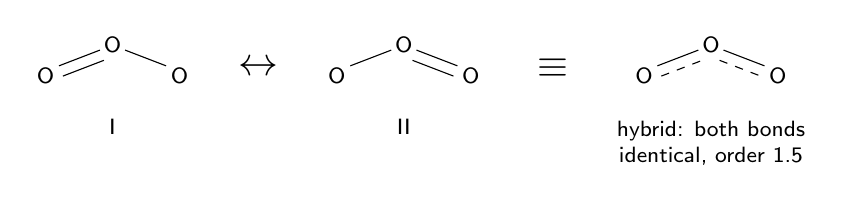
\begin{tikzpicture}[font=\sffamily\footnotesize]
  % structure I
  \node at (-0.85,0.5) {O}; \node at (0,0.9) {O}; \node at (0.85,0.5) {O};
  \draw (-0.68,0.63) -- (-0.16,0.83);
  \draw (-0.63,0.5) -- (-0.11,0.7);
  \draw (0.16,0.83) -- (0.68,0.63);
  \node at (0,-0.15) {I};
  % arrow
  \node[font=\Large] at (1.85,0.6) {$\leftrightarrow$};
  % structure II
  \begin{scope}[xshift=3.7cm]
    \node at (-0.85,0.5) {O}; \node at (0,0.9) {O}; \node at (0.85,0.5) {O};
    \draw (-0.16,0.83) -- (-0.68,0.63);
    \draw (0.16,0.83) -- (0.68,0.63);
    \draw (0.11,0.7) -- (0.63,0.5);
    \node at (0,-0.15) {II};
  \end{scope}
  % arrow to hybrid
  \node[font=\Large] at (5.6,0.6) {$\equiv$};
  % hybrid
  \begin{scope}[xshift=7.6cm]
    \node at (-0.85,0.5) {O}; \node at (0,0.9) {O}; \node at (0.85,0.5) {O};
    \draw (-0.68,0.63) -- (-0.16,0.83);
    \draw[dashed] (-0.63,0.5) -- (-0.11,0.7);
    \draw (0.16,0.83) -- (0.68,0.63);
    \draw[dashed] (0.11,0.7) -- (0.63,0.5);
    \node[align=center] at (0,-0.35) {hybrid: both bonds\\identical,
      order 1.5};
  \end{scope}
\end{tikzpicture}
\end{center}

\begin{apctrap}
The molecule does \textbf{not} flip between the structures. A resonance
hybrid is one unchanging species whose electrons are
\term{delocalized}; the separate drawings are a limitation of Lewis
notation, not a description of anything happening in time.
\end{apctrap}

\begin{workedexample}[I do: what resonance predicts, and how we know]
\textbf{Ozone, \ce{O3}}, has 18 valence electrons and can be drawn with
the double bond on either side. Neither drawing alone is right.

\textbf{The prediction.} If the true structure is an average, the two
\ce{O-O} bonds must be \textbf{identical} --- each one and a half bonds
--- with a length between a single and a double bond.

\textbf{The evidence.} A pure \ce{O-O} single bond is about
\SI{148}{\pico\meter} and a pure \ce{O=O} double bond about
\SI{121}{\pico\meter}. Both bonds in ozone measure
\SI{128}{\pico\meter} --- equal to each other, and between the two
reference values. Exactly what the hybrid predicts and what neither
individual structure predicts.

\textbf{Nitrate does the same thing.} \ce{NO3-} has three equivalent
structures, so all three \ce{N-O} bonds are identical with bond order
$4/3$. Had the ion really contained one double and two single bonds, one
bond would be measurably shorter --- and it is not.

\textbf{Bond order in a hybrid:} total bonds shared, divided by the
number of positions. Ozone: 3 bonds over 2 positions $= 1.5$. Nitrate:
4 over 3 $\approx 1.33$.
\end{workedexample}

\begin{yourturn}[YOUR TURN 9 --- four questions]
\begin{enumerate}[leftmargin=*,itemsep=0.5em]
  \item How many resonance structures does \ce{SO2} have, and what is
        its \ce{S-O} bond order? \workspace[1.6cm]
  \item The carbonate ion \ce{CO3^2-} has three equivalent structures.
        Give the \ce{C-O} bond order. \workspace[1.6cm]
  \item Predict how the three \ce{C-O} bond lengths in carbonate
        compare, and why. \workspace[1.6cm]
  \item A student says ozone ``rapidly switches between its two
        structures''. Correct them. \workspace[1.8cm]
\end{enumerate}
\selfcheck{(a) two; order 1.5 \quad (b) $4/3 \approx 1.33$ \quad
(c) all three identical \quad (d) it does not switch --- the electrons
are delocalized}
\keyonly{\begin{apcanswer}(a) \textbf{Two} equivalent structures; 3 bonds
over 2 positions gives bond order \textbf{1.5}, and the two \ce{S-O}
bonds are equal. (b) 4 bonds shared over 3 positions:
$\mathbf{4/3 \approx 1.33}$. (c) \textbf{All three identical}, and
intermediate between a \ce{C-O} single and a \ce{C=O} double bond. That
is the measurable prediction of the hybrid, and it is what experiment
finds. (d) There is \textbf{no switching}. Ozone is a single species
whose $\pi$ electrons are \textbf{delocalized} over all three oxygens at
once. The two drawings are an artefact of Lewis notation, which can only
place a bond in one location at a time; the molecule itself never
changes.\end{apcanswer}}
\end{yourturn}

% =====================================================================
\section*{\sffamily Ladder 10 \textbullet\ VSEPR: predicting shape}
\zsec{8.13}

Electron domains --- bonds (single, double or triple each count once)
and lone pairs --- repel and get as far apart as possible. Count the
domains on the central atom and the geometry follows.

\begin{center}
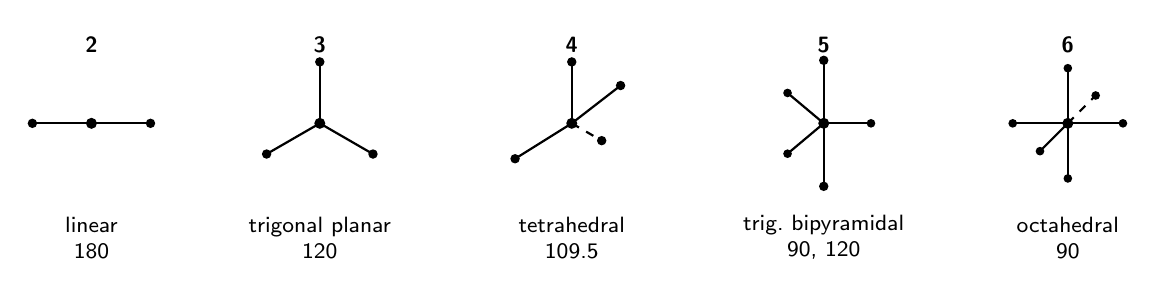
\begin{tikzpicture}[font=\sffamily\footnotesize]
  % 2 linear
  \node at (0,1.5) {\textbf{2}};
  \node (c) at (0,0.5) {};
  \fill (0,0.5) circle (0.07);
  \draw[thick] (-0.75,0.5) -- (0.75,0.5);
  \fill (-0.75,0.5) circle (0.06); \fill (0.75,0.5) circle (0.06);
  \node[align=center] at (0,-0.95) {linear\\\SI{180}{\degree}};

  % 3 trigonal planar
  \begin{scope}[xshift=2.9cm]
    \node at (0,1.5) {\textbf{3}};
    \fill (0,0.5) circle (0.07);
    \foreach \a in {90,210,330} {
      \draw[thick] (0,0.5) -- ++(\a:0.78);
      \fill ([shift={(0,0.5)}]\a:0.78) circle (0.06);}
    \node[align=center] at (0,-0.95) {trigonal planar\\\SI{120}{\degree}};
  \end{scope}

  % 4 tetrahedral
  \begin{scope}[xshift=6.1cm]
    \node at (0,1.5) {\textbf{4}};
    \fill (0,0.5) circle (0.07);
    \draw[thick] (0,0.5) -- (0,1.28); \fill (0,1.28) circle (0.06);
    \draw[thick] (0,0.5) -- (-0.72,0.05); \fill (-0.72,0.05) circle (0.06);
    \draw[thick,dashed] (0,0.5) -- (0.38,0.28); \fill (0.38,0.28) circle (0.06);
    \draw[thick] (0,0.5) -- (0.62,0.98); \fill (0.62,0.98) circle (0.06);
    \node[align=center] at (0,-0.95) {tetrahedral\\\SI{109.5}{\degree}};
  \end{scope}

  % 5 trigonal bipyramidal
  \begin{scope}[xshift=9.3cm]
    \node at (0,1.5) {\textbf{5}};
    \fill (0,0.5) circle (0.07);
    \draw[thick] (0,0.5) -- (0,1.3); \fill (0,1.3) circle (0.06);
    \draw[thick] (0,0.5) -- (0,-0.3); \fill (0,-0.3) circle (0.06);
    \foreach \a in {0,140,220} {
      \draw[thick] (0,0.5) -- ++(\a:0.6);
      \fill ([shift={(0,0.5)}]\a:0.6) circle (0.055);}
    \node[align=center] at (0,-0.95) {trig.\ bipyramidal\\90,
      \SI{120}{\degree}};
  \end{scope}

  % 6 octahedral
  \begin{scope}[xshift=12.4cm]
    \node at (0,1.5) {\textbf{6}};
    \fill (0,0.5) circle (0.07);
    \foreach \a in {0,90,180,270} {
      \draw[thick] (0,0.5) -- ++(\a:0.7);
      \fill ([shift={(0,0.5)}]\a:0.7) circle (0.055);}
    \draw[thick,dashed] (0,0.5) -- ++(45:0.5);
    \fill ([shift={(0,0.5)}]45:0.5) circle (0.055);
    \draw[thick] (0,0.5) -- ++(225:0.5);
    \fill ([shift={(0,0.5)}]225:0.5) circle (0.055);
    \node[align=center] at (0,-0.95) {octahedral\\\SI{90}{\degree}};
  \end{scope}
\end{tikzpicture}
\end{center}

\textbf{Lone pairs are the twist.} They occupy a domain and set the
\emph{electron} geometry, but you cannot see them --- the
\emph{molecular} shape names only the atoms. And because a lone pair is
held by one nucleus rather than shared between two, it spreads out more
and \textbf{squeezes the bond angles down}:

\begin{center}
\begin{tikzpicture}[font=\sffamily\footnotesize]
  \foreach \x/\f/\lp/\ang in {0/\ce{CH4}/0/109.5, 4.1/\ce{NH3}/1/107,
                              8.2/\ce{H2O}/2/104.5} {
    \node[font=\sffamily\small] at (\x,1.5) {\f};
    \node at (\x,1.05) {\lp\ lone pair(s)};
    \fill (\x,0.4) circle (0.07);
    \draw[thick] (\x,0.4) -- ++(-125:0.72);
    \draw[thick] (\x,0.4) -- ++(-55:0.72);
    \draw[{Stealth[length=2mm]}-{Stealth[length=2mm]}]
      ([shift={(\x,0.4)}]-125:0.42) arc (-125:-55:0.42);
    \node at (\x,-0.55) {\SI{\ang}{\degree}};}
  \draw[-{Stealth[length=3mm]},thick,apcgray] (0.9,-1.05) -- (7.3,-1.05);
  \node[below,font=\sffamily\small] at (4.1,-1.1)
    {more lone pairs \textbullet\ more compression \textbullet\ smaller
     angle};
\end{tikzpicture}
\end{center}

\begin{workedexample}[I do: four domains, three different shapes]
All three molecules below have \textbf{four} electron domains, so all
three have a \textbf{tetrahedral electron geometry}. Their molecular
shapes differ entirely.

\begin{center}
\renewcommand{\arraystretch}{1.25}
\begin{tabular}{@{}lllll@{}}
\hline
& \textbf{Bonds} & \textbf{Lone pairs} & \textbf{Molecular shape} &
  \textbf{Angle} \\
\hline
\ce{CH4} & 4 & 0 & tetrahedral & \SI{109.5}{\degree} \\
\ce{NH3} & 3 & 1 & trigonal pyramidal & \SI{107}{\degree} \\
\ce{H2O} & 2 & 2 & bent & \SI{104.5}{\degree} \\
\hline
\end{tabular}
\end{center}

\textbf{Why the angle shrinks down the column.} A bonding pair is shared
between two nuclei, which holds it in a relatively narrow region. A lone
pair answers to only one nucleus, so it spreads wider and pushes harder
on everything around it. One lone pair compresses the remaining angles a
little; two compress them more.

\textbf{Why the shape names differ.} Electron geometry counts all four
domains; molecular shape names only where the \emph{atoms} are. You
cannot see a lone pair, so \ce{H2O} is called bent, not tetrahedral ---
even though its four domains are arranged tetrahedrally.
\end{workedexample}

\begin{yourturn}[YOUR TURN 10 --- four questions]
\begin{enumerate}[leftmargin=*,itemsep=0.5em]
  \item Domains, electron geometry, and molecular shape for \ce{BF3}.
        \workspace[1.6cm]
  \item Same three for \ce{SO2} (one lone pair on S). \workspace[1.6cm]
  \item Same three for \ce{CO2}. \workspace[1.6cm]
  \item \ce{PCl3} and \ce{BCl3} both have three bonded atoms, but only
        one is polar. Which, and why? \workspace[1.8cm]
\end{enumerate}
\selfcheck{(a) 3, trigonal planar, trigonal planar \quad (b) 3, trigonal
planar, bent \quad (c) 2, linear, linear \quad (d) \ce{PCl3} --- it has
a lone pair, so it is pyramidal and the dipoles do not cancel}
\keyonly{\begin{apcanswer}(a) \textbf{3} domains, no lone pairs:
electron geometry \textbf{trigonal planar}, molecular shape
\textbf{trigonal planar}, \SI{120}{\degree}. (b) \textbf{3} domains (two
bonds, one lone pair): electron geometry \textbf{trigonal planar},
molecular shape \textbf{bent} at slightly under \SI{120}{\degree}.
(c) \textbf{2} domains --- each double bond counts once: electron
geometry and molecular shape are both \textbf{linear} at
\SI{180}{\degree}. (d) \textbf{\ce{PCl3}}. Phosphorus has a lone pair, so
the molecule is trigonal \textbf{pyramidal} and the three \ce{P-Cl}
dipoles do not cancel. Boron has none, so \ce{BCl3} is trigonal
\textbf{planar} and symmetric, and its three dipoles sum to zero. Same
number of bonded atoms, opposite polarity --- decided entirely by the
lone pair.\end{apcanswer}}
\end{yourturn}

% =====================================================================
\section*{\sffamily Mastery tracker}

Tick a row only if \textbf{all four} YOUR TURN questions were right on
the first attempt.

\renewcommand{\arraystretch}{1.35}
\noindent\begin{tabular}{@{}c p{6.2cm} c p{4.8cm}@{}}
\toprule
\textbf{First try?} & \textbf{Skill} & \textbf{Ladder} &
  \textbf{If not, re-read\ldots}\\
\midrule
$\square$ & bond type from $\Delta$EN & 1 & the scale is a guideline \\
$\square$ & molecular polarity & 2 & bonds AND shape \\
$\square$ & ion sizes, isoelectronic & 3 & same electrons, count protons \\
$\square$ & lattice energy & 4 & charge first, size as tie-breaker \\
$\square$ & bond energies and $\Delta H$ & 5 & broken minus formed \\
$\square$ & Lewis structures & 6 & the electron count is the check \\
$\square$ & octet exceptions & 7 & expansion needs period 3 \\
$\square$ & formal charge & 8 & closest to zero wins \\
$\square$ & resonance & 9 & one hybrid, not switching \\
$\square$ & VSEPR & 10 & electron vs molecular geometry \\
\bottomrule
\end{tabular}

\begin{apcnote}[Scoring yourself honestly]
10/10: this chapter feeds Unit 2 directly, and Ladders 6--10 are the ones
the exam draws on most heavily.

7--9: redo the missed ladders tomorrow, not today.

6 or fewer: the misses almost always cluster in one of two places.
If they are in Ladders 3--5, the problem is \emph{explanation} --- you
are reaching for octets and stability where the answer must name a
charge, a distance, or a shielding difference. If they are in Ladders
6--10, the problem is \emph{procedure}, and the fix is mechanical:
redraw every Lewis structure in the chapter from a blank page, counting
electrons at the start and checking the total at the end. Those are
different problems with different fixes --- diagnose which one you have
before redoing anything.
\end{apcnote}

\end{document}
